\documentclass[a4paper]{article}
\usepackage{ccs2022,color}

\begin{document}

\title{Template of abstract for the congress CCS2022}

\author{
First Author$^1$,
\underline{Presenting Author}$^2$,	%Underline the presenting author.
\and
Third Author$^1$
\\
$^1$First institution name, first institution address
\\
$^2$Second institution name, second institution address
}
\maketitle

% Uncomment next line for switch off column balancing (only if you have problems with column balancing).
%\raggedcolsend\raggedend

% Body text %%%%%%%%%%%%%%%%%%%%%%%%%%%%%%%%%%%%%%%%%%%%%%%%%%%%%%%%%%%%%
Use this template to prepare your abstract.
{\bf The length of the document must be of \underline{one page} and it must contain at least one figure.}  
You can add references following standard formats \cite{journal.cite,book.cite}.
Figures must be included in \texttt{pdf} (see Fig.~\ref{fig1} for an example).
You can type inline equations $E_n = \hbar\omega(n + 1/2)$, and also displayed equations
\begin{equation}
E_n = \hbar\omega\left( n + \frac{1}{2} \right),
\label{eq:harmonic.oscillator}
\end{equation}
as in the case of Eq.~(\ref{eq:harmonic.oscillator}).
Once written the abstract and compiled, please save a pdf version and upload it in the easychair web page of CCS2022 \cite{easy}. You can find the link and the instructions under the call for abstracts in the CCS web \cite{web}. The information you will be asked includes the names and emails of the authors, the presenting author, and the track of the conference you are submitting to. The list of tracks is:
\begin{itemize}
\setlength\itemsep{-0.4em}
\item Foundations of Complex Systems. Basic Sciences. Quantum complexity;
\item Complex Networks;
\item Data Science, Machine Learning and Artificial Intelligence in the context of Complex Systems;
\item Computation and information processing in complex systems;
\item Economics and Finance;
\item Social systems;
\item Ecological systems;
\item Cognition, psychology and neurosciences;
\item Complexity in Biology and Health Sciences;
\item City Science, Mobility and Transport;
\item Energy, Environment, Sustainability, Climate and Global change.
\end{itemize} 

New paragraphs should be slightly indented (latex does it by default). You can continue writing new text and including new equations
\begin{equation}
\label{eq2}
\phi = m\, \psi,
\end{equation}
the numbering is automatic but please remember to add labels if you cite them in the text using {\tt $\backslash$eqref\{label\} } as in \eqref{eq2}.

Figures must be included in vectorial (pdf, eps, etc) or non-vectorial (png, jpg, etc) format (see Fig. \ref{fig1} for an example). In this latter case, the resolution of the images should be as high as possible. 300 dpi would be optimal but it can be lower to avoid massive final pdf file sizes but never below 70 dpi. Note that at least one figure is required. The format of the references should follow the examples given below, with the title of the papers as optional depending on space availability.  


% Figures %%%%%%%%%%%%%%%%%%%%%%%%%%%%%%%%%%%%%%%%%%%%%%%%%%%%%%%%%%%%%%%
\begin{figure}[H]
\begin{center}
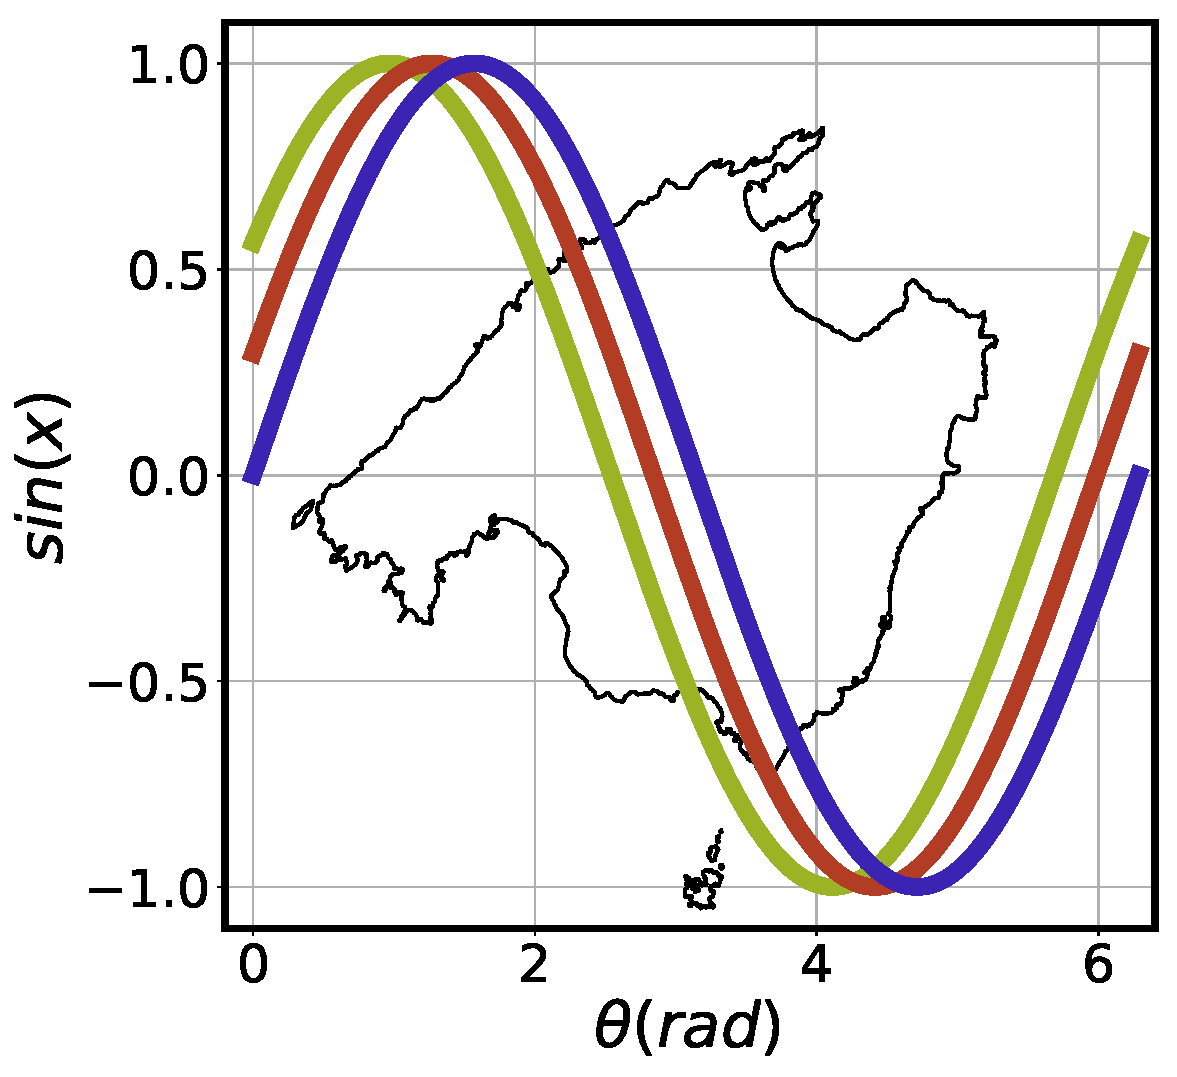
\includegraphics[width=8cm]{figure1}
\caption{Include here the figure caption.}
\label{fig1}
\end{center}
\end{figure}
%%%%%%%%%%%%%%%%%%%%%%%%%%%%%%%%%%%%%%%%%%%%%%%%%%%%%%%%%%%%%%%%%%%%%%%%%

% References %%%%%%%%%%%%%%%%%%%%%%%%%%%%%%%%%%%%%%%%%%%%%%%%%%%%%%%%%%%%
\footnotesize
\begin{thebibliography}{9}
\bibitem{journal.cite} A.~Author1, B.~Author2, and C.~Author3, \emph{Title of article can optionally be included}, J.\ Comp.\ Sys.\ \textbf{10}, 1820 (2018).
\bibitem{book.cite} A.~A.~Author1 and B.~B.~Author2, \emph{Procs. of the WWW'2028 or book title}, (Palma, 2028).
\bibitem{easy} {\color{blue} \underline{https://easychair.org/conferences/?conf=ccs2022} }
\bibitem{web}  {\color{blue} \underline{https://www.ccs2022.org} }
\end{thebibliography}

\end{document}
